%!TEX root = ../main.tex

\subsubsection{High Level CAN protocol}\label{sub:CAN_protocol}
Due to the requirements of the on-kart network, it is decided to formulate a new protocol specifically for this project. The requirements are listed below.\\
\paragraph{On-kart network requirements:}
\begin{itemize}
	\item Simple and easy to learn.
	\item Support for 16 nodes.
	\item One node must be able to receive/transmit data to/from multiple inputs/outputs
	\item Publish/subscribe architecture.
	\item Variable data length - beyond 8 bytes per message
	\item Expandable -- must be able to add more nodes without affecting the existing ones.
	\item Commands: Start/stop broadcasting 
	\item Commands can be send to specific or all nodes
\end{itemize}

\label{sub:CANopen}
As mentioned before, CANopen is a high level protocol that runs on top of the CAN protocol.
It is open source project, that runs on the top 5 layers of the OSI model\cite{CANopen_introduction}, and is governed by the Can in Automation (CiA) group.
It includes several types of protocols, most interesting are the SDO and PDO. 
By splitting the 11 bit Message ID into a 4 bit function code, followed by 7 bits of node ID, meaning that a node can communicate 16 different functions to 127 different nodes.\\
The Service Data Object (SDO) can read from or write to any registers on any node. 
It can handle 127 different nodes with each 65536 different indices, each with 256 sub indices -- in all more than 2 billion addresses with each 4 bytes of data.
The way CANopen supports this, is by using the first four bytes of the data portion of the frame for metadata, as described in figure~\ref{fig:CANopen_SDO_data}.

\begin{figure}[h]
	\centering
	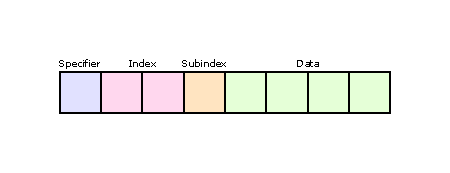
\includegraphics[width=0.9\linewidth]{graphics/CANopen_SDO_data}
	\caption{"The data section of the CAN frame is split into three parts: one byte for the specifier, three bytes for the node index and subindex, and four bytes for the actual data in the transfer."\cite{CANopen_introduction}}
	\label{fig:CANopen_SDO_data}
\end{figure}

This of course means that the overhead from one message increases from 47 bits to 59 bits, or 184 \% of the maximum data size.\\
This protocol is not ideal for this network. 
In part because it's request based, but more because of the enormous overhead -- the IMU would produce 999 bits in order to transmit its 9 axis data without loss of precision, and at 400 Hz, that node alone will take up 40 \% of the bandwidth.
In addition to this, all transmits would need to be requested, so the total bandwidth comes close to 70 \%.
%Metadata is 47 bits, plus 32 bits from the Data portion. The data it self is a float, so that's 32 bits; 111 in all. A request does not include data, so that's only 79 bits of data. At 400 Hz, that's (111+79)*9*400=684000.
The SDO is generally used to define or read parameters for that node, that are not bound to change over time.
It should not be used for broadcasting data.

The Process Data Object (PDO) is a protocol used to transmit specific indices with a higher throughput. 
In this protocol, certain indices are mapped to one of 8 PDOs. 
This way, a node can identify data only by the CAN message ID, without using any of the data portion for overhead.
It is also possible to group multiple values together, and to transmit without request -- either at fixed time or event driven.
This brings the data from the IMU down to 523 bits to transmit its 9 axis data.\\
%((32+32)+47)*4+(47+32)

Each device on the CANopen bus has its own Object Dictionary (OD) specifying its addresses. 
Some of these addresses are reserved, but since the Message ID specifies which node it is, there's no risk of overlapping. 
However if two nodes need to communicate meaningful data -- i.e. data that the receiving node needs as an input, and not just something it writes into a log file -- they need to know about portions of each other's OD, or at least the PDO.
If then one part is replaced by a different make or model, then it might be necessary to reconfigure other nodes, and the system loses modularity.\\

For all its nice features, the CANopen protocols do not fit the requirements outlined in the beginning of this section. 
On one hand it supports way more nodes than is needed, but does not support enough data producing or data consuming subnodes.
It also includes a lot of complexity, which is not needed for this project, and that only adds unnecessary compleixity. 
Instead it has been decided to develop a custom High Level Protocol that relies more on the automatic functionality of the CAN protocol.\\

The basic CAN framework is retained for this protocol, and the protocol is really just a naming convention for the message ID. 

\begin{figure}[h!]
	\centering
	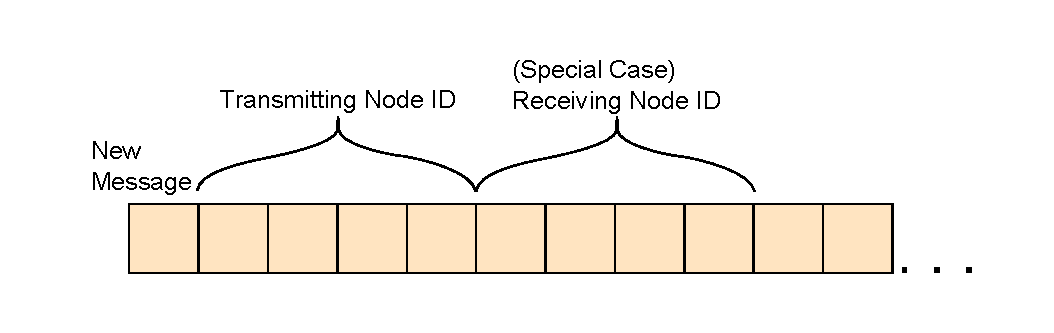
\includegraphics[width = 0.9\linewidth]{graphics/CAN_protocol_general_pdf}
	\caption{Naming convention for this high level protocol}
	\label{fig:CAN_protocol_general_pdf}
\end{figure}

The message ID is split in to three portions, as seen on figure~\ref{fig:CAN_protocol_general_pdf}.
The first bit is set to 1 if this is a new message.
If however the node needs to send more than 8 bytes in one package, this bit can be set to 0, thus blocking other nodes with higher priority.
The subsequent four bits indicate the transmitting node ID, which will allow up to 16 nodes. 
The last 6 bits of the message ID would determine the message type.
This message type then determines 
This leaves 64 different message types for each node -- it is then the developers to utilize these the best. 
If more message types are needed, the CAN protocol supports extended identifier, which adds 18 bits of identifiers.
This however also increases the overhead, and puts unnecessary load on the bus
Each node will have a list of message IDs (10 bits), that it knows how to handle.
If a message is not on that list, the node will ignore it.\\

There are basically two types of nodes: The Wifi node acting as a commander, and all other nodes.
Generally nodes can either produce data, and/or receive commands.
The Wifi node neither produces any kind of data nor receives commands, but it does receive data, and send out commands.
Therefore, there is a special case, for when the Wifi node is sending.
In this case, the subsequent four bits determines the recipient, leaving two bits for command type. 
For now, command types are only "Start broadcasting" and "Stop broadcasting", but could be extended to for instance "Set parameter" or "Set value", where the data field will indicate which parameter, and what is's set to.
If the recipient message ID is the WiFi node ID, then the command applies to all nodes.\\

The four node IDs are:
\begin{table}[h]
	\begin{tabular}{{l} {l}}
		Wifi node: & 0b0001 \\
		IMU node: & 0b0011 \\
		Sevcon node: & 0b0111 \\
		GPS node: & 0b1110
	\end{tabular}
\end{table}

The reason for this naming is, that the Wifi node acts as a commander for the, and it's commands need higher priority.
The IMU produces short data packages at a high rate, and the GPS node produces longer data packages at a lower rate. 
Therefore it is of less concern if the GPS message is delayed due to obstruction from other nodes. 

\subsubsection{Publisher-Subscriber Architecture}
\catalin{Should I explain more about the architecture? Or is it the readers responsibility to read about it?}
A mechanism was also necessary to control the receivers and transmitters of messages.
One of the functionalities of the network was to provide the ability for various nodes to be able to send specific messages to other nodes.
Such a mechanism could easily be implemented using the Publisher-Subscriber architecture which would also make the network data-driven.
Using this method, the communication among the various nodes could be easily configured just by adding messages ids to an array variable containing the node's subscriptions.
The use of this architecture was incorporated in the protocol functionality, along with a set of functions in the source code.
\paragraph{Implementation in code}~\\
This was achieved by implementing a set of functions and an array variable of subscriptions for each node.
The important mechanisms that needed to be provided by the source code were the creation of the message id, the decoding of it as well as getting the various portions such as the node id and the message type.
\\
The figure \ref{fig:SeqDiagram_SendFrame} shows the procedure of sending a frame to the CAN network containing data, which makes use of the protocol function createMsgID().
After returning the message id, the id and the data are put into the TxFrame to be sent once the FIFO has space.
The actual sending is done with a call to the XCanPs function XCanPs\_Send().
\\
Similarly, the procedure of receiving a frame is shown in the figure \ref{fig:SeqDiagram_RecvFrame}.
The node once it calls the RecvFrame() function, it waits in a loop until it receives a frame. Then, it checks the subscriptions in order to forward the packet for further processing or to ignore it.

\begin{figure}[h!]
	\centering
	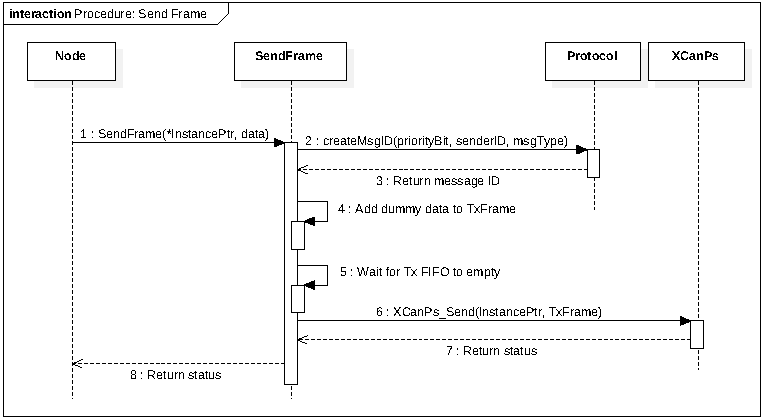
\includegraphics[width = 1.1\linewidth]{graphics/SeqDiagram_SendFrame.pdf}
	\caption{The sequence diagram of the process of sending a frame.}
	\label{fig:SeqDiagram_SendFrame}
\end{figure}

\begin{figure}[h!]
	\centering
	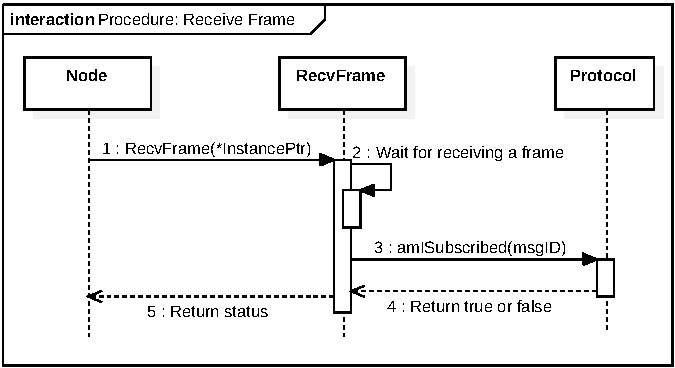
\includegraphics[width = 1.1\linewidth]{graphics/SeqDiagram_RecvFrame.pdf}
	\caption{The sequence diagram of the process of receiving a frame.}
	\label{fig:SeqDiagram_RecvFrame}
\end{figure}